% ============================================================
% Figure 2: HAA-RAG Pipeline (similar to RoboDexVLM Fig.2 working pipeline)
% Shows the three-level hierarchical retrieval process
% Compile: pdflatex fig_haarag_pipeline.tex
% ============================================================
\documentclass[border=3pt]{standalone}
\usepackage{tikz}
\usetikzlibrary{
  positioning, arrows.meta, shapes.geometric, shapes.multipart,
  fit, backgrounds, calc, decorations.pathreplacing, patterns,
  shadows.blur
}
\usepackage{xcolor}
\usepackage{times}
\usepackage{amsmath,amssymb}

% Colors
\definecolor{querybg}{HTML}{EBF5FB}
\definecolor{querybdr}{HTML}{2E86C1}
\definecolor{l1bg}{HTML}{FEF9E7}
\definecolor{l1bdr}{HTML}{F39C12}
\definecolor{l2bg}{HTML}{EAFAF1}
\definecolor{l2bdr}{HTML}{27AE60}
\definecolor{l3bg}{HTML}{F4ECF7}
\definecolor{l3bdr}{HTML}{8E44AD}
\definecolor{kbbg}{HTML}{FDEBD0}
\definecolor{kbbdr}{HTML}{E67E22}
\definecolor{outbg}{HTML}{FADBD8}
\definecolor{outbdr}{HTML}{E74C3C}
\definecolor{textgray}{HTML}{5D6D7E}
\definecolor{matchgreen}{HTML}{27AE60}
\definecolor{failred}{HTML}{E74C3C}

\begin{document}
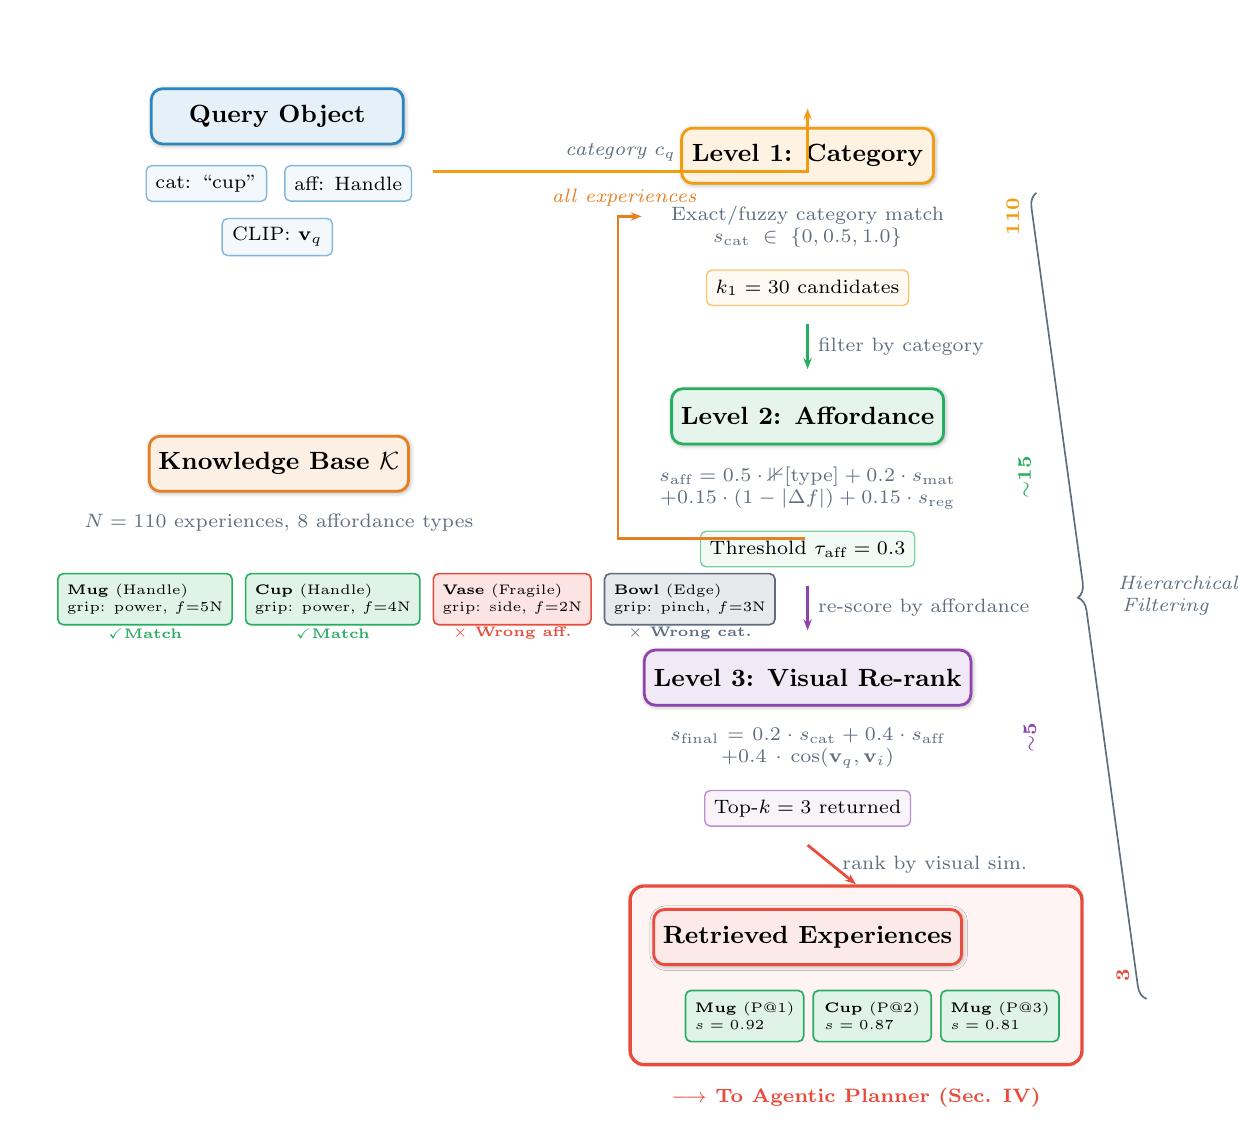
\begin{tikzpicture}[
  >=Stealth,
  node distance=0.3cm,
  block/.style={
    rectangle, rounded corners=4pt,
    draw=#1, fill=#1!12, line width=1pt,
    minimum width=3.2cm, minimum height=0.7cm,
    font=\small\bfseries, text=black, align=center,
    blur shadow={shadow blur steps=4, shadow xshift=0.4pt, shadow yshift=-0.4pt}
  },
  smallblock/.style={
    rectangle, rounded corners=2pt,
    draw=#1!60, fill=#1!6, line width=0.5pt,
    minimum width=1.4cm, minimum height=0.45cm,
    font=\scriptsize, text=black, align=center
  },
  expcard/.style={
    rectangle, rounded corners=2pt,
    draw=#1, fill=#1!15, line width=0.6pt,
    minimum width=1.5cm, minimum height=0.65cm,
    font=\tiny, text=black, align=left
  },
  myarrow/.style={
    ->, line width=1pt, color=#1,
    >={Stealth[length=4pt, width=3pt]}
  },
  levelbox/.style 2 args={
    rectangle, rounded corners=5pt,
    draw=#1, fill=#2, line width=1.2pt,
    inner sep=7pt
  }
]

% ================================================================
% QUERY INPUT (top-left)
% ================================================================
\node[block=querybdr] (query) {Query Object};
\node[smallblock=querybdr, below=0.25cm of query, xshift=-0.9cm] (qcat) {cat: ``cup''};
\node[smallblock=querybdr, below=0.25cm of query, xshift=0.9cm] (qaff) {aff: Handle};
\node[smallblock=querybdr, below=0.2cm of qcat, xshift=0.9cm] (qvis) {CLIP: $\mathbf{v}_q$};

\begin{scope}[on background layer]
  \node[levelbox={querybdr}{querybg!40}, fit=(query)(qcat)(qaff)(qvis),
    label={[font=\footnotesize\bfseries, text=querybdr]above:{Input: RGB-D + Instruction}}] (querybox) {};
\end{scope}

% ================================================================
% KNOWLEDGE BASE (left column)
% ================================================================
\node[block=kbbdr, below=2cm of querybox] (kb) {Knowledge Base $\mathcal{K}$};
\node[font=\scriptsize, text=textgray, below=0.15cm of kb] (kbinfo) {$N=110$ experiences, 8 affordance types};

% Experience cards
\node[expcard=matchgreen, below=0.4cm of kbinfo, xshift=-1.7cm] (e1) 
  {\textbf{Mug} (Handle)\\grip: power, $f$=5N};
\node[expcard=matchgreen, right=0.15cm of e1] (e2) 
  {\textbf{Cup} (Handle)\\grip: power, $f$=4N};
\node[expcard=failred, right=0.15cm of e2] (e3) 
  {\textbf{Vase} (Fragile)\\grip: side, $f$=2N};
\node[expcard=textgray, right=0.15cm of e3] (e4) 
  {\textbf{Bowl} (Edge)\\grip: pinch, $f$=3N};

% Match/Fail indicators
\node[font=\tiny\bfseries, text=matchgreen] at ($(e1.south)+(0,-0.1)$) {\checkmark Match};
\node[font=\tiny\bfseries, text=matchgreen] at ($(e2.south)+(0,-0.1)$) {\checkmark Match};
\node[font=\tiny\bfseries, text=failred] at ($(e3.south)+(0,-0.1)$) {$\times$ Wrong aff.};
\node[font=\tiny\bfseries, text=textgray] at ($(e4.south)+(0,-0.1)$) {$\times$ Wrong cat.};

\begin{scope}[on background layer]
  \node[levelbox={kbbdr}{kbbg!30}, fit=(kb)(kbinfo)(e1)(e2)(e3)(e4), inner sep=10pt,
    yshift=-3pt] (kbbox) {};
\end{scope}

% ================================================================
% THREE RETRIEVAL LEVELS (right column, vertical)
% ================================================================

% Level 1: Category
\node[block=l1bdr, right=3.5cm of query, yshift=-0.5cm] (l1) {Level 1: Category};
\node[font=\scriptsize, text=textgray, below=0.15cm of l1, text width=3.5cm, align=center] (l1desc) 
  {Exact/fuzzy category match\\$s_{\text{cat}} \in \{0, 0.5, 1.0\}$};
\node[smallblock=l1bdr, below=0.15cm of l1desc] (l1result)
  {$k_1=30$ candidates};
  
\begin{scope}[on background layer]
  \node[levelbox={l1bdr}{l1bg!40}, fit=(l1)(l1desc)(l1result), inner sep=6pt] (l1box) {};
\end{scope}

% Level 2: Affordance
\node[block=l2bdr, below=0.8cm of l1box] (l2) {Level 2: Affordance};
\node[font=\scriptsize, text=textgray, below=0.15cm of l2, text width=3.8cm, align=center] (l2desc) 
  {$s_{\text{aff}} = 0.5 \cdot \mathbb{1}[\text{type}] + 0.2 \cdot s_{\text{mat}}$\\
  $+ 0.15 \cdot (1-|\Delta f|) + 0.15 \cdot s_{\text{reg}}$};
\node[smallblock=l2bdr, below=0.15cm of l2desc] (l2result)
  {Threshold $\tau_{\text{aff}}=0.3$};
  
\begin{scope}[on background layer]
  \node[levelbox={l2bdr}{l2bg!40}, fit=(l2)(l2desc)(l2result), inner sep=6pt] (l2box) {};
\end{scope}

% Level 3: Visual Re-rank
\node[block=l3bdr, below=0.8cm of l2box] (l3) {Level 3: Visual Re-rank};
\node[font=\scriptsize, text=textgray, below=0.15cm of l3, text width=3.8cm, align=center] (l3desc) 
  {$s_{\text{final}} = 0.2 \cdot s_{\text{cat}} + 0.4 \cdot s_{\text{aff}}$\\
  $+ 0.4 \cdot \cos(\mathbf{v}_q, \mathbf{v}_i)$};
\node[smallblock=l3bdr, below=0.15cm of l3desc] (l3result)
  {Top-$k=3$ returned};
  
\begin{scope}[on background layer]
  \node[levelbox={l3bdr}{l3bg!40}, fit=(l3)(l3desc)(l3result), inner sep=6pt] (l3box) {};
\end{scope}

% ================================================================
% OUTPUT (bottom-right)
% ================================================================
\node[block=outbdr, below=0.8cm of l3box] (output) {Retrieved Experiences};
\node[expcard=matchgreen, below=0.3cm of output, xshift=-0.8cm] (out1)
  {\textbf{Mug} (P@1)\\$s=0.92$};
\node[expcard=matchgreen, right=0.1cm of out1] (out2)
  {\textbf{Cup} (P@2)\\$s=0.87$};
\node[expcard=matchgreen, right=0.1cm of out2] (out3)
  {\textbf{Mug} (P@3)\\$s=0.81$};

\begin{scope}[on background layer]
  \node[levelbox={outbdr}{outbg!30}, fit=(output)(out1)(out2)(out3), inner sep=8pt] (outbox) {};
\end{scope}

% ================================================================
% ARROWS
% ================================================================
% Query -> Level 1
\draw[myarrow=l1bdr] (querybox.east) -| (l1box.north)
  node[near start, above, font=\scriptsize\itshape, text=textgray] {category $c_q$};

% Level 1 -> Level 2
\draw[myarrow=l2bdr] (l1box.south) -- (l2box.north)
  node[midway, right, font=\scriptsize, text=textgray] {filter by category};

% Level 2 -> Level 3
\draw[myarrow=l3bdr] (l2box.south) -- (l3box.north)
  node[midway, right, font=\scriptsize, text=textgray] {re-score by affordance};

% Level 3 -> Output
\draw[myarrow=outbdr] (l3box.south) -- (outbox.north)
  node[midway, right, font=\scriptsize, text=textgray] {rank by visual sim.};

% KB -> Level 1 (retrieve)
\draw[myarrow=kbbdr, line width=0.8pt] (kbbox.east) -| ($(l1box.west)+(-0.3, 0)$) -- (l1box.west)
  node[near start, above, font=\scriptsize\itshape, text=kbbdr] {all experiences};

% Output -> Planner (usage arrow)
\node[font=\scriptsize\bfseries, text=outbdr, below=0.15cm of outbox] (tolabel) 
  {$\longrightarrow$ To Agentic Planner (Sec. IV)};

% ================================================================
% Decorative: Funnel shape annotation
% ================================================================
\node[font=\scriptsize\bfseries, text=l1bdr, rotate=90] at ($(l1box.east)+(0.5, 0)$) {110};
\node[font=\scriptsize\bfseries, text=l2bdr, rotate=90] at ($(l2box.east)+(0.5, 0)$) {$\sim$15};
\node[font=\scriptsize\bfseries, text=l3bdr, rotate=90] at ($(l3box.east)+(0.5, 0)$) {$\sim$5};
\node[font=\scriptsize\bfseries, text=outbdr, rotate=90] at ($(outbox.east)+(0.5, 0)$) {3};

% Funnel bracket
\draw[decorate, decoration={brace, amplitude=5pt, mirror}, line width=0.6pt, textgray] 
  ($(l1box.east)+(0.8, 0.3)$) -- ($(outbox.east)+(0.8, -0.3)$)
  node[midway, right=6pt, font=\scriptsize\itshape, text=textgray, text width=1.2cm, align=center] 
  {Hierarchical\\Filtering};

\end{tikzpicture}
\end{document}
